188. \begin{figure}[ht!]
\center{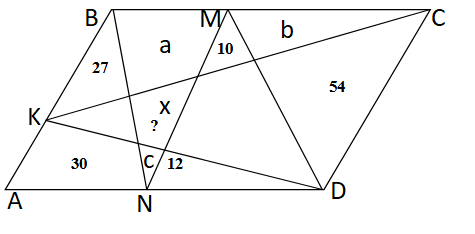
\includegraphics[scale=0.6]{g8-188.png}}
\end{figure}\\
Так как формула нахождения площади треугольника отличается от формулы нахождения площади параллелограмма только множителем $\cfrac{1}{2},$ имеем равенства
$\cfrac{1}{2}S_{ABCD}=S_{\Delta BKC}+S_{\Delta AKD}=S_{\Delta BMN}+S_{\Delta CMD},$ откуда $27+a+10+b+30+c+12=a+x+c+b+54,\ x=25.$\\
